\documentclass[final,3p]{elsarticle}

%% Use the option review to obtain double line spacing
%% \documentclass[preprint,review,12pt]{elsarticle}

%% Use the options 1p,twocolumn; 3p; 3p,twocolumn; 5p; or 5p,twocolumn
%% for a journal layout:
%% \documentclass[final,1p,times]{elsarticle}
%% \documentclass[final,1p,times,twocolumn]{elsarticle}
%% \documentclass[final,3p,times]{elsarticle}
%% \documentclass[final,3p,times,twocolumn]{elsarticle}
%% \documentclass[final,5p,times]{elsarticle}
%% \documentclass[final,5p,times,twocolumn]{elsarticle}

\usepackage{hyperref}
\usepackage[capitalize]{cleveref}

%% if you use PostScript figures in your article
%% use the graphics package for simple commands
%% \usepackage{graphics}
%% or use the graphicx package for more complicated commands
\usepackage{graphicx}
%% or use the epsfig package if you prefer to use the old commands
%% \usepackage{epsfig}

\usepackage{caption,subcaption}
\usepackage{float}

%% The amssymb package provides various useful mathematical symbols
\usepackage{amssymb}
%% The amsthm package provides extended theorem environments
%% \usepackage{amsthm}

%% The lineno packages adds line numbers. Start line numbering with
%% \begin{linenumbers}, end it with \end{linenumbers}. Or switch it on
%% for the whole article with \linenumbers after \end{frontmatter}.
%% \usepackage{lineno}
\usepackage{amsmath}
\usepackage{xfrac}

% Modify citation style.
\usepackage[numbers]{natbib}

% Packages for custom table views.
% The multirow package provides merged row cells, while booktabs allows customizing the lines.
\usepackage{multirow, booktabs}
% These packages allow colors in table.
\usepackage{color, colortbl}

% Chinese support
\usepackage{xeCJK}
\setCJKmainfont{Lantinghei TC}

%% natbib.sty is loaded by default. However, natbib options can be
%% provided with \biboptions{...} command. Following options are
%% valid:

%%   round  -  round parentheses are used (default)
%%   square -  square brackets are used   [option]
%%   curly  -  curly braces are used      {option}
%%   angle  -  angle brackets are used    <option>
%%   semicolon  -  multiple citations separated by semi-colon
%%   colon  - same as semicolon, an earlier confusion
%%   comma  -  separated by comma
%%   numbers-  selects numerical citations
%%   super  -  numerical citations as superscripts
%%   sort   -  sorts multiple citations according to order in ref. list
%%   sort&compress   -  like sort, but also compresses numerical citations
%%   compress - compresses without sorting
%%
%% \biboptions{comma,round}

% \biboptions{}

\journal{LS1012 General Biology Lab, 106-1}

% adjust the footer
\makeatletter
\def\ps@pprintTitle{%
 \let\@oddhead\@empty%
 \let\@evenhead\@oddhead
 \def\@oddfoot{\centerline{\thepage}}%
 \let\@evenfoot\@oddfoot}
\makeatother

% custom color
\definecolor{Gray}{gray}{0.9}

\begin{document}

\begin{frontmatter}

\title{作業四 Generative Adversarial Networks}

\author{劉彥廷~B03902036}

\end{frontmatter}

%%
%% Start line numbering here if you want
%%
% \linenumbers

\section{模型敘述}
	以下為本次作業採用的模型預覽
	\begin{figure}[H]
		\centering
		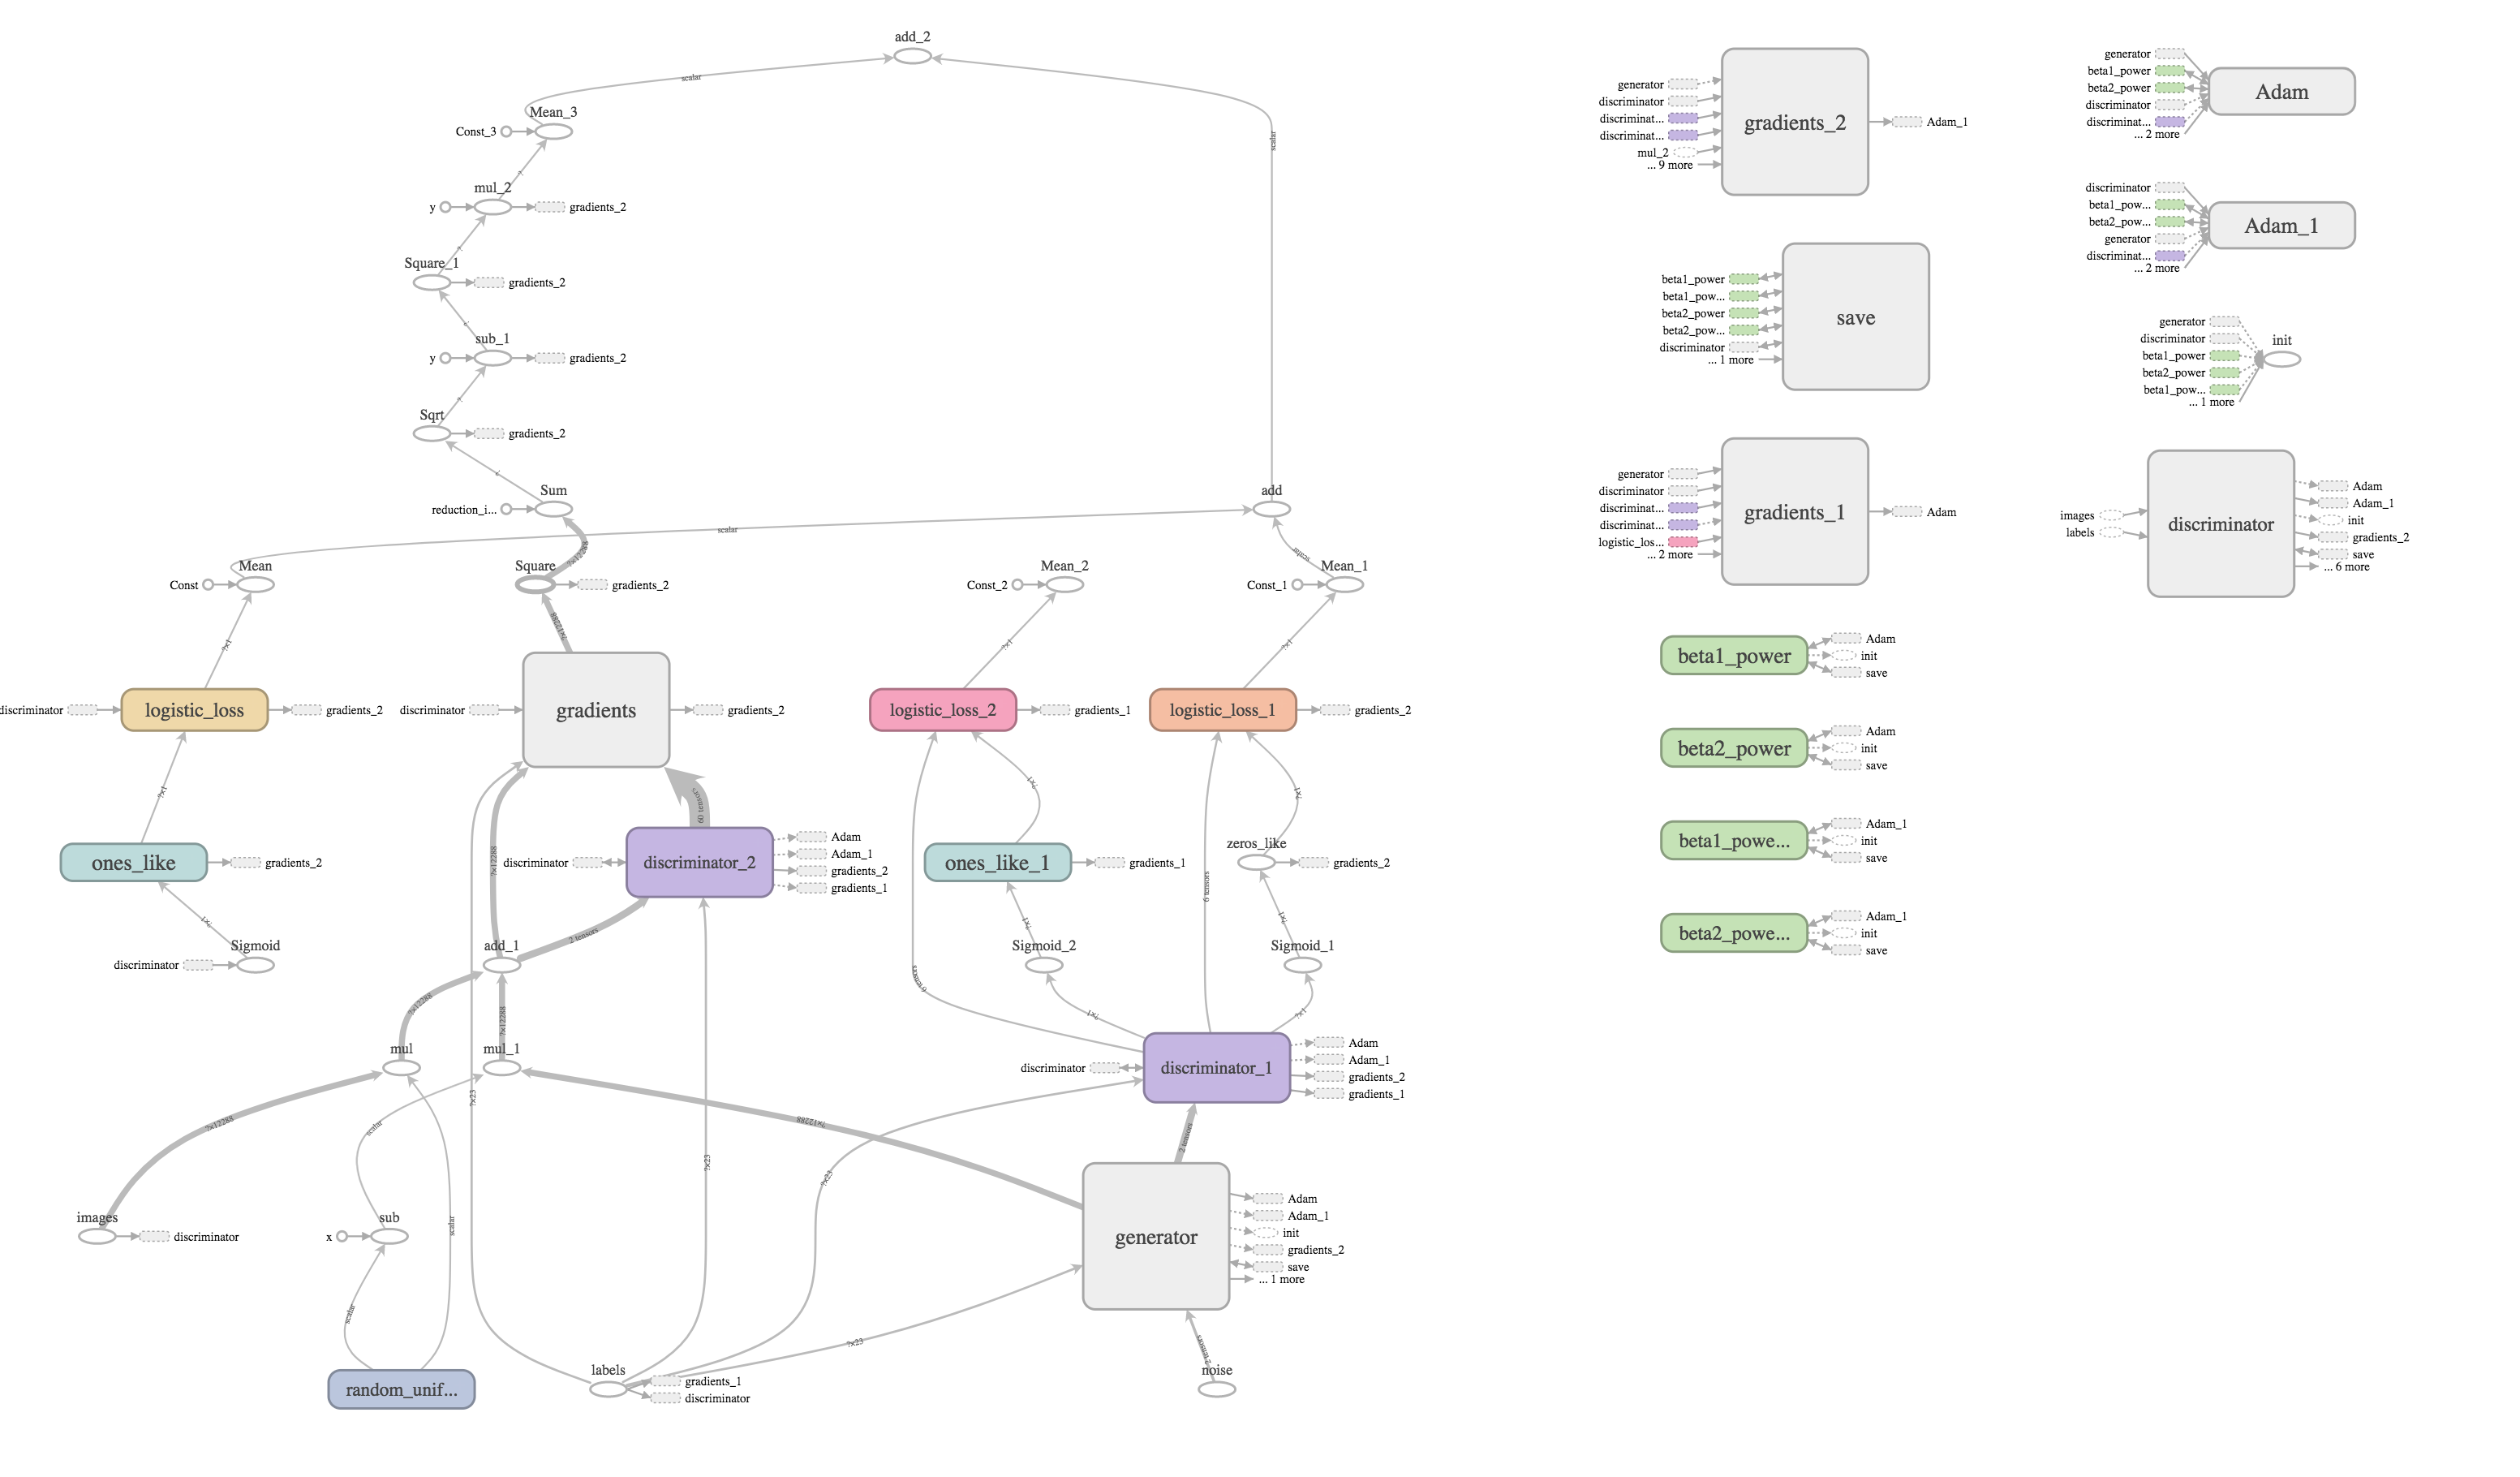
\includegraphics[width=0.95\textwidth]{images/model}
		\label{fig:model}
	\end{figure}
	其本質上為 conditional WGAN-GP(使用了 gradient penalty 的 WGAN)。
	文字的編碼直接採用助教會評量的 23 種 tags 構成的 one-hot vector。
	吐出的影像為 64x64 的結果。
	
	根據報告規範,要寫出 loss functions
	\begin{equation*}
		L^{WGAN-GP}_{D} = E \lbrack D(x) \rbrack - E \lbrack D(G(z)) \rbrack - \lambda E \lbrack ( \Vert \nabla D(\epsilon x + (1-\epsilon) G(z) )\Vert -1)^2 \rbrack
	\end{equation*}
	其中 $\lambda$ 在程式裡頭為 scale 此一變數。
	\begin{equation*}
		L^{WGAN-GP}_{G} = E \lbrack D(G(z)) \rbrack
	\end{equation*}
	
\section{效能改善}
	最開始的時候參考了 \cite{jiamings91:online} 與 \cite{zhangqia0:online} 實作了 Conditional WGAN。
	但在調整 generator 與 discriminator 的更新比例(以下簡稱 D/G 比)時,出現了 mode collapse 且收斂時間很久,所以轉而更新模型為 Conditional WGAN-GP(WGAN 換為投影片當中的 Improved WGAN)。
	\begin{figure}[H]
		\centering
		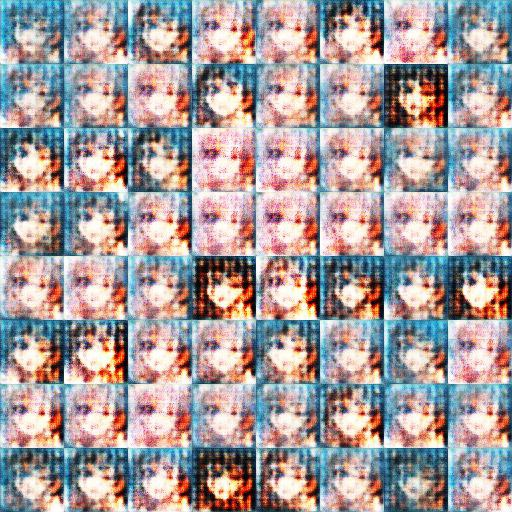
\includegraphics[width=0.48\textwidth]{images/wgan_d1_g5_900}
		\caption{WGAN 的 D/G 比 0.2 發生的 mode collapse} 
	\end{figure}
	
	
	以下為 WGAN 與 WGAN-GP 兩者之間的 G loss 與 D loss 比較。
	\begin{figure}[H]
		\centering
		\begin{subfigure}{.48\textwidth}
			\centering
			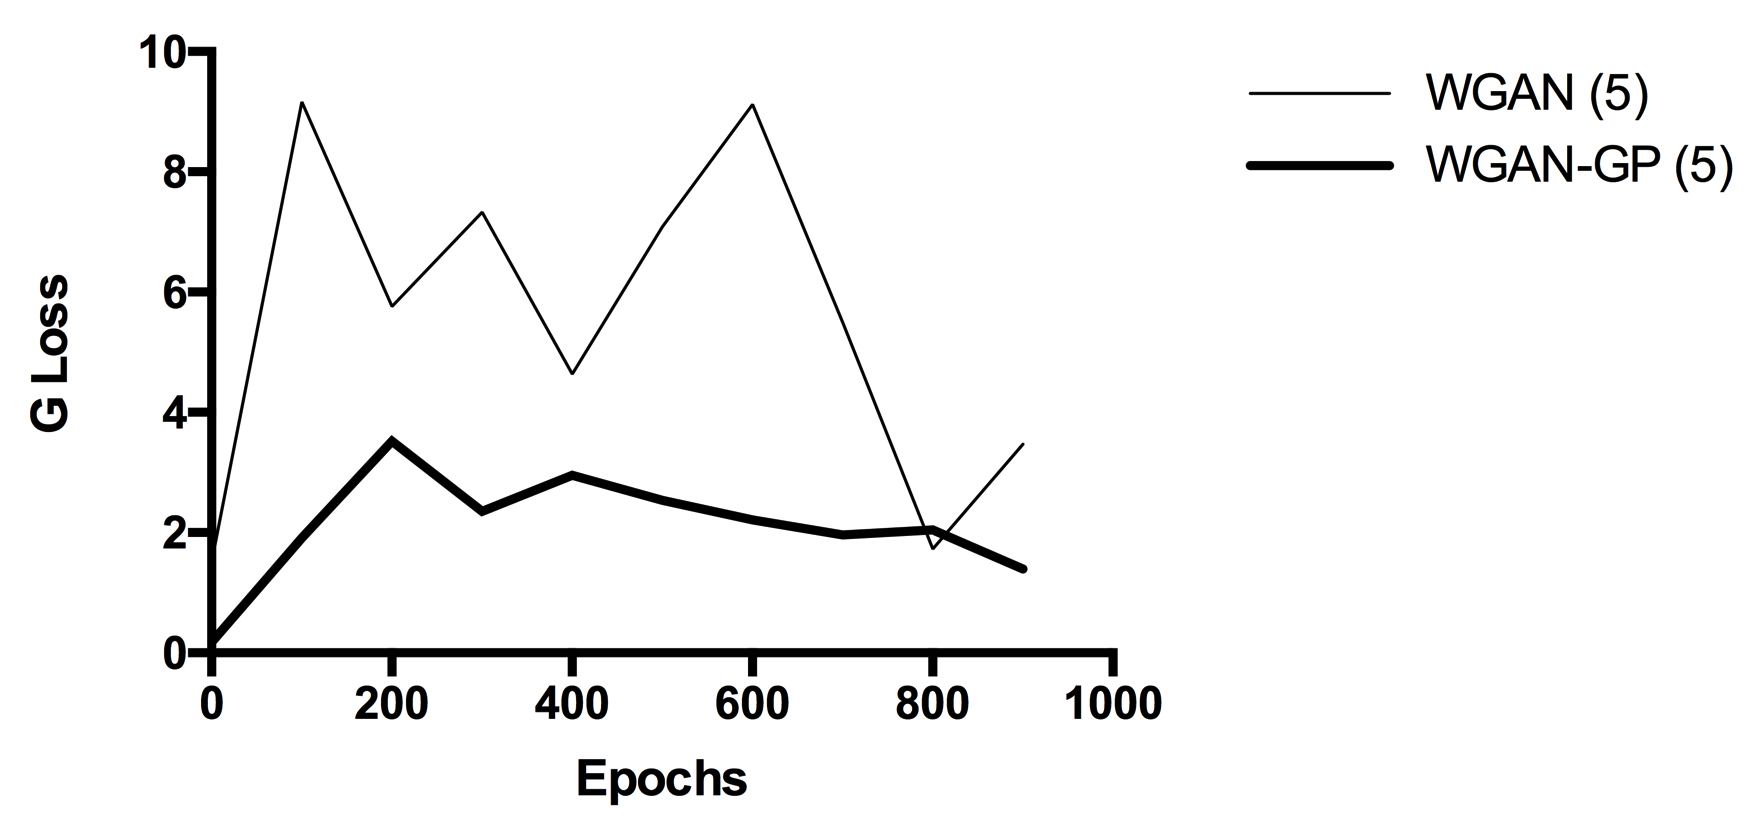
\includegraphics[width=\linewidth]{images/g_loss_wgangp}
			\caption{G loss}
		\end{subfigure}
		~
		\begin{subfigure}{.48\textwidth}
			\centering
			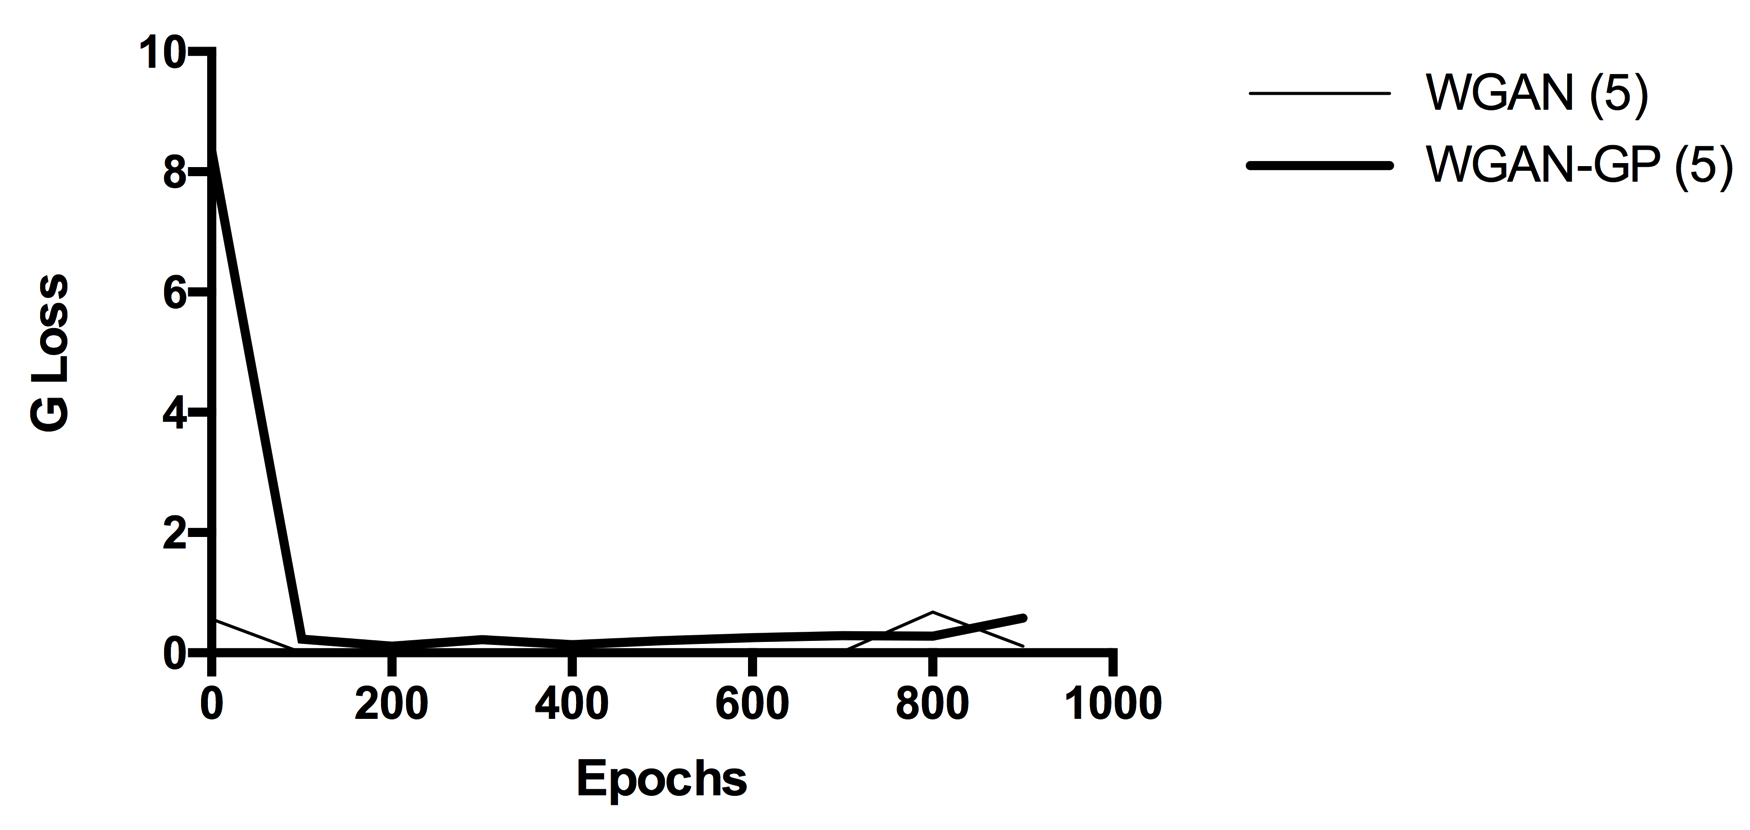
\includegraphics[width=\linewidth]{images/d_loss_wgangp}
			\caption{D loss}
		\end{subfigure}
		\label{fig:dg_gd_loss}
	\end{figure}

\section{實驗設置與觀察}
	最終繳交的模型每更新 5 次 discriminator 就會更新 1 次 generator,該模型總共經歷過了 10000 次這個循環。
	
	\begin{figure}[H]
		\centering
		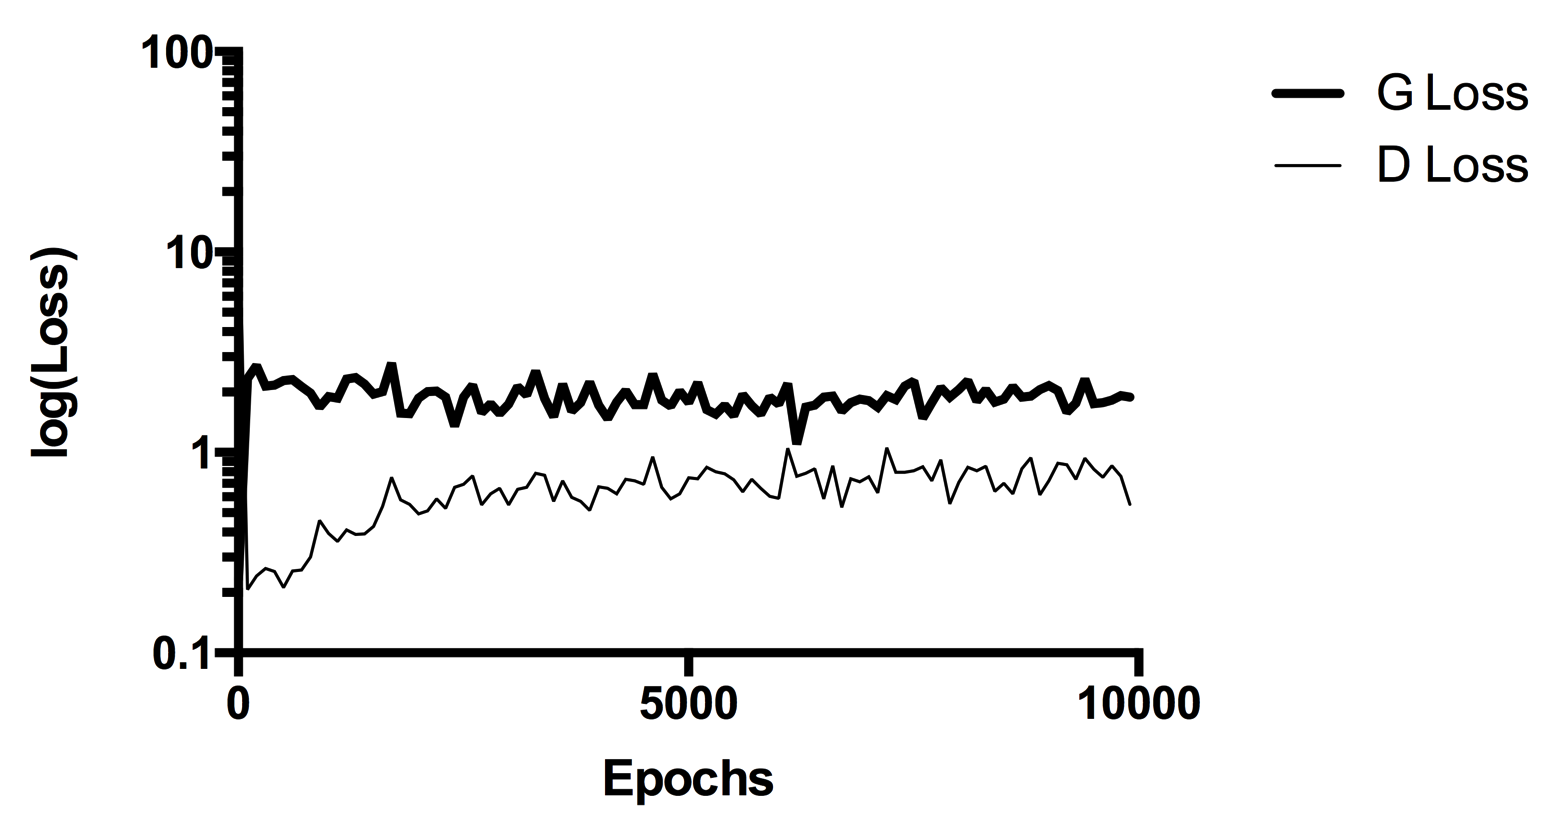
\includegraphics[width=0.48\textwidth]{images/wgan_gp_loss}
		\caption{WGAN-GP 的 log loss} \label{fig:wgan_gp_loss}
	\end{figure}
	
	以下為最後的結果
	\begin{figure}[H]
		\centering
		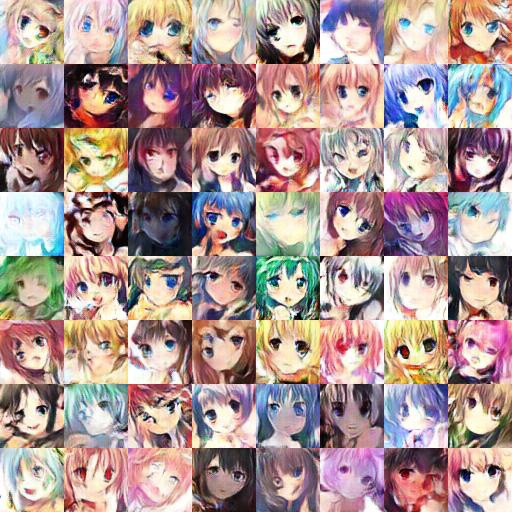
\includegraphics[width=0.48\textwidth]{images/wgan_gp_9900_montage}
	\end{figure}
	
	在本次作業當中針對 WGAN 實驗了不同的更新比例並觀察其 loss。
	D/G 比變高代表了 discriminator 有比較多的時間學習,loss 預期會下降,反之則為 generator 的 loss 下降。
	\begin{figure}[H]
		\centering
		\begin{subfigure}{.48\textwidth}
			\centering
			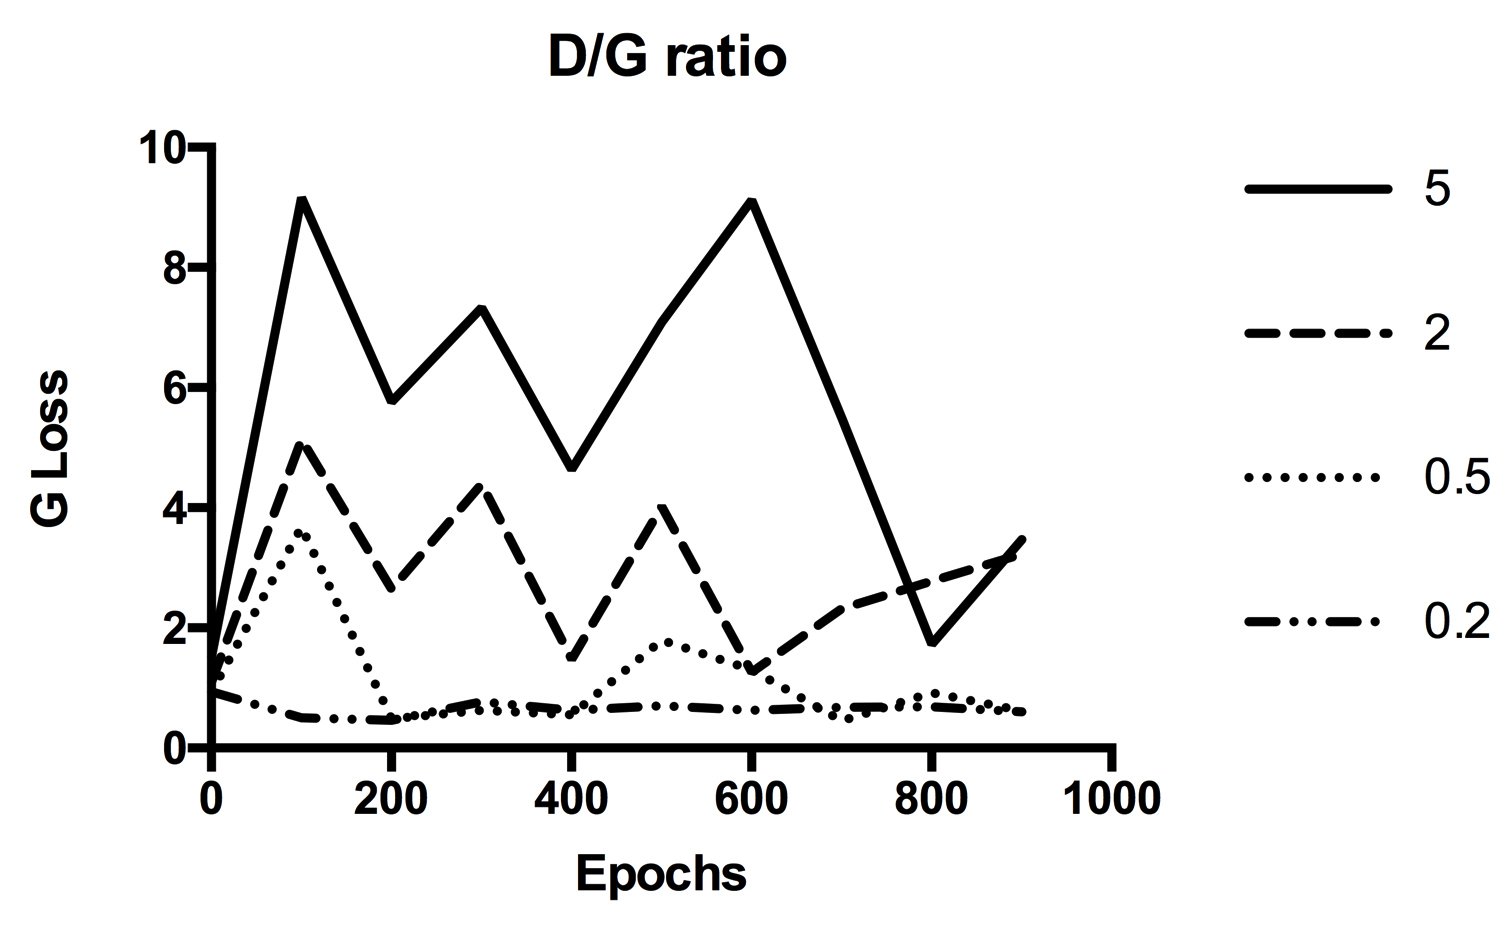
\includegraphics[width=\linewidth]{images/g_loss_dg}
			\caption{G loss}
		\end{subfigure}
		~
		\begin{subfigure}{.48\textwidth}
			\centering
			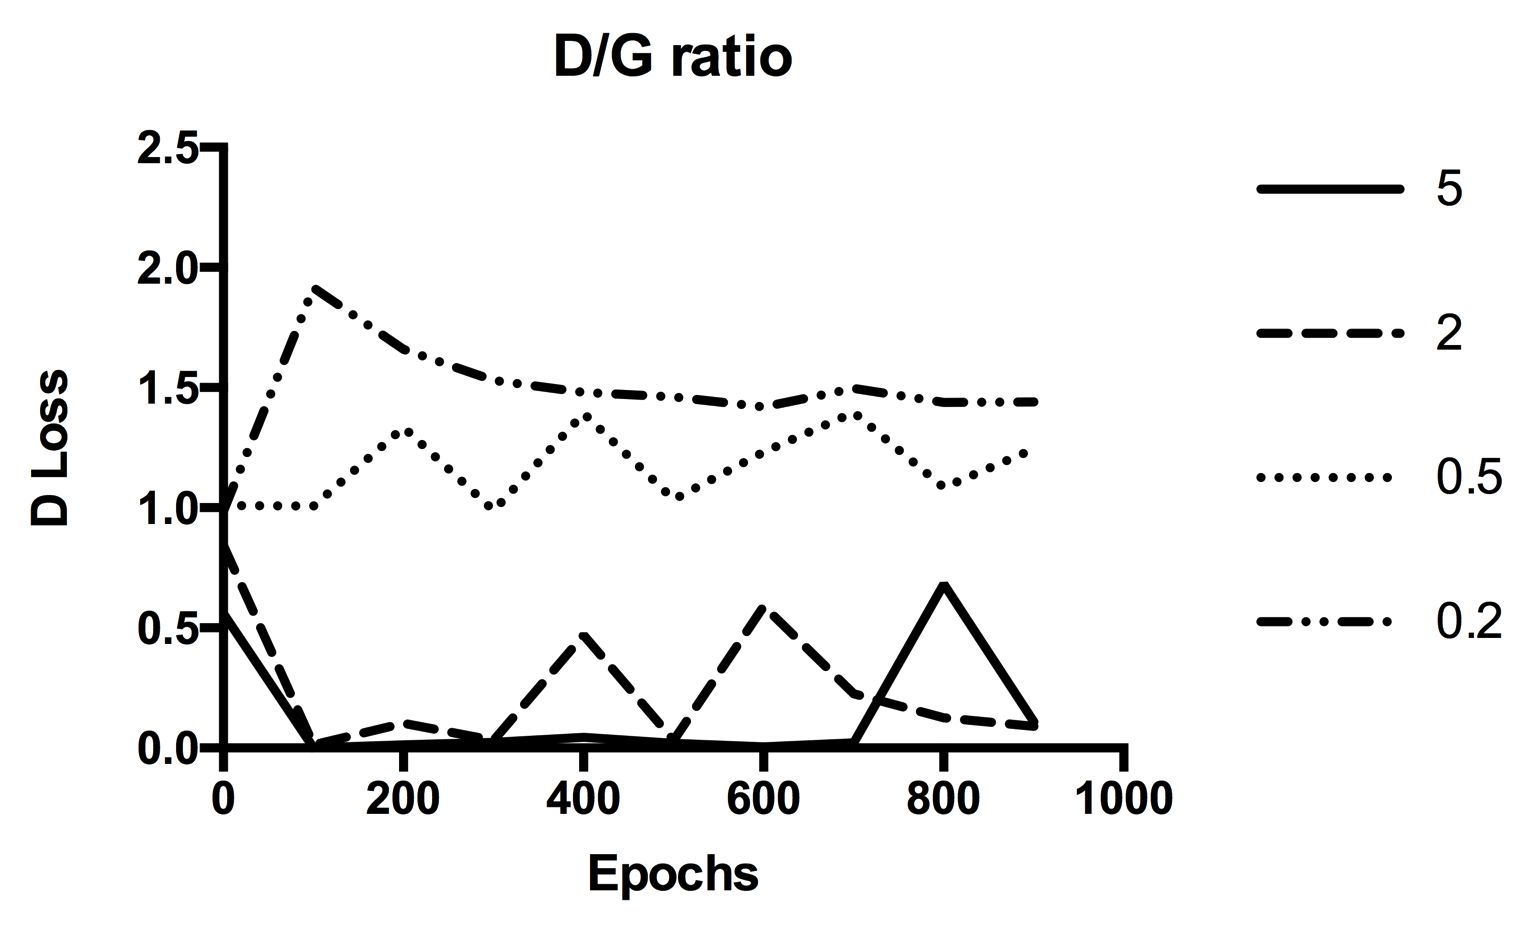
\includegraphics[width=\linewidth]{images/d_loss_dg}
			\caption{D loss}
		\end{subfigure}
		\label{fig:dg_loss}
	\end{figure}
	
	但有趣的是,先更新 generator 似乎 loss 都會相較於先更新 discriminator 來得高。
	推測是基於 discriminator 後更新的話,在剛開始的 epochs 當中,generator 的表現會變差因為錯誤的判決,而錯誤不斷累積最終造成了整體的 GAN 表現不佳。
	\begin{figure}[H]
		\centering
		\begin{subfigure}{.48\textwidth}
			\centering
			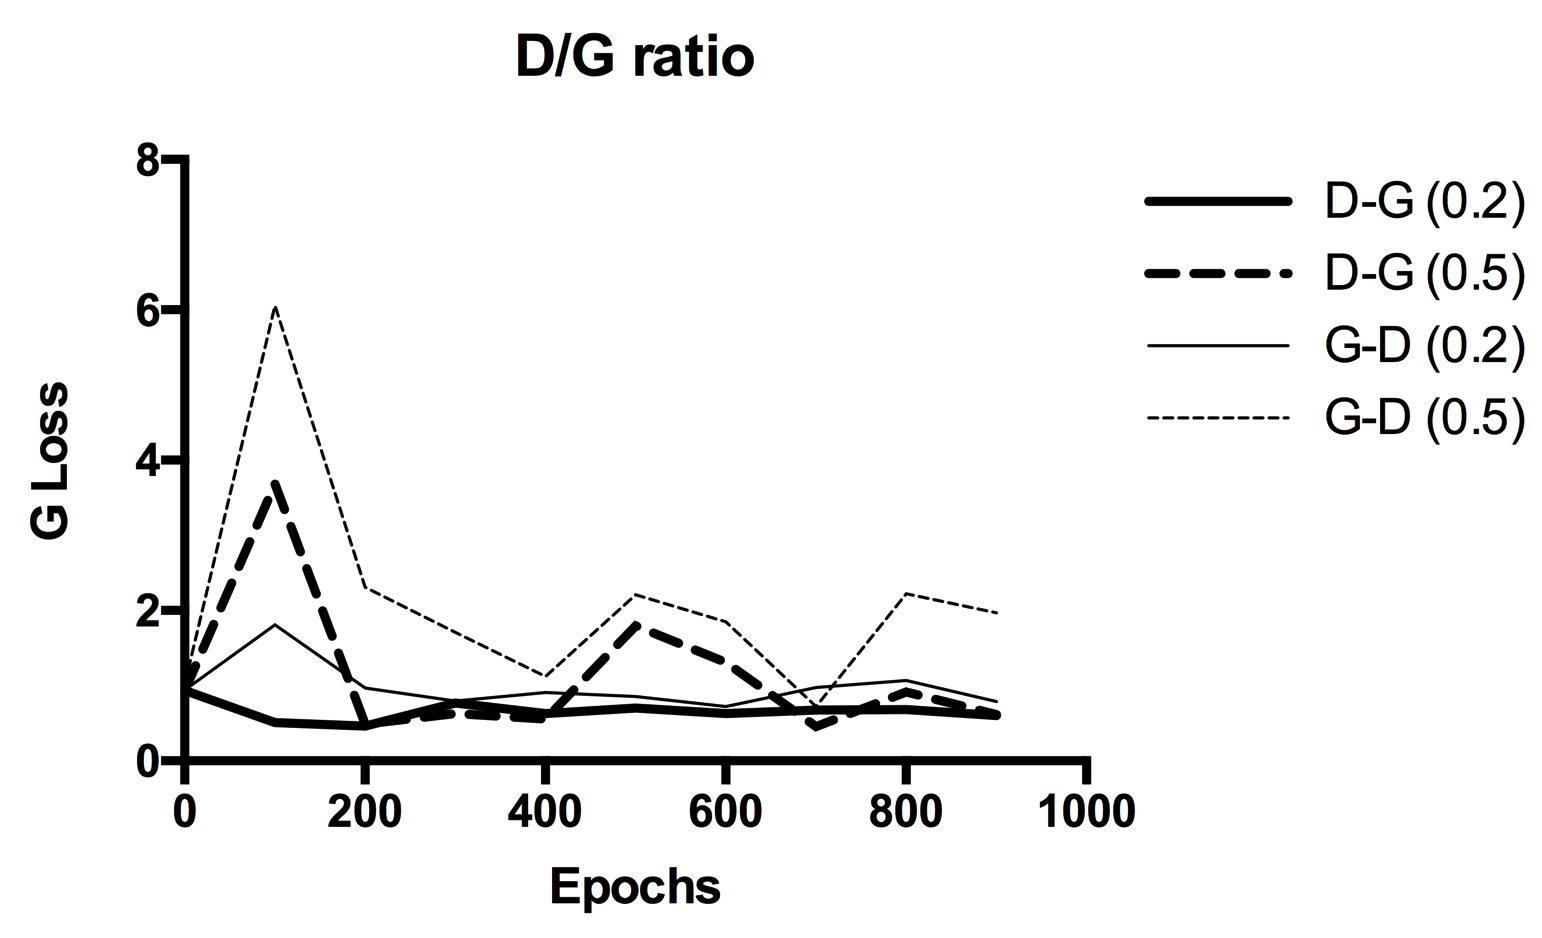
\includegraphics[width=\linewidth]{images/g_loss_dg_gd}
			\caption{G loss}
		\end{subfigure}
		~
		\begin{subfigure}{.48\textwidth}
			\centering
			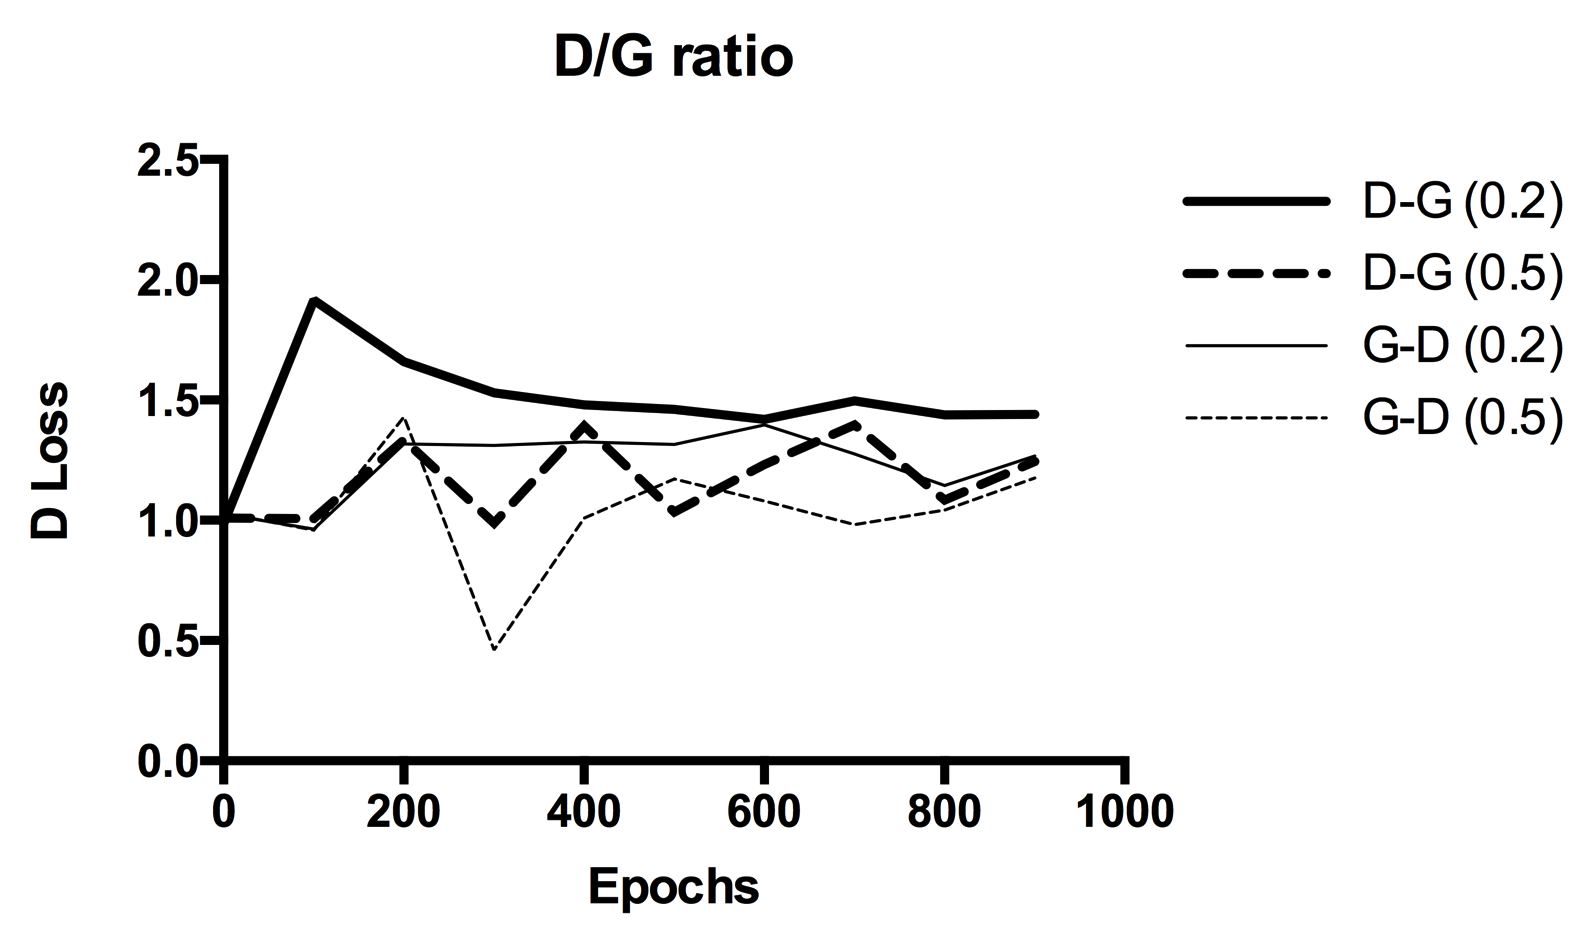
\includegraphics[width=\linewidth]{images/d_loss_dg_gd}
			\caption{D loss}
		\end{subfigure}
		\label{fig:dg_gd_loss}
	\end{figure}
		
%% References
%%
%% Following citation commands can be used in the body text:
%% Usage of \cite is as follows:
%%   \cite{key}         ==>>  [#]
%%   \cite[chap. 2]{key} ==>> [#, chap. 2]
%%

\nocite{Wasserst52:online} 

%% References with bibTeX database:
\bibliographystyle{apa}

\section{參考文獻}
\bibliography{reference}

%% The Appendices part is started with the command \appendix;
%% appendix sections are then done as normal sections
% Have the appendices start with a new page.
%\newpage
%\appendix
	
\end{document}
